% Citations should be in bibtex format and go in references.bib
\documentclass[a4paper, 11pt]{article}
\usepackage[top=3cm, bottom=3cm, left = 2cm, right = 2cm]{geometry} 
\geometry{a4paper} 
\usepackage[utf8]{inputenc}
\usepackage{textcomp}
\usepackage{graphicx} 
\usepackage{amsmath,amssymb}  
\usepackage{bm}  
\usepackage[pdftex,bookmarks,colorlinks,breaklinks]{hyperref}  
\hypersetup{linkcolor=black,citecolor=black,filecolor=black,urlcolor=black} % black links, for printed output
\usepackage{memhfixc} 
\usepackage{pdfsync}  

\begin{document}
	\begin{titlepage}
		\renewcommand{\baselinestretch}{0.5}
		\thispagestyle{empty}
		\begin{center}
			\Huge
			\textsc{Fakulta informačných technologií\\[5pt]VUT v~Brne}\\
			\vspace{\stretch{0.382}}
			\huge Parallel K\,--\,Means algorithm\\
			\Large PRL project 2
			\vspace{\stretch{0.618}}
		\end{center}
		{
			\Large \today \hfill Peter Močáry (xmocar00)
		}
	\end{titlepage}

\newpage
\tableofcontents
\newpage
\setcounter{page}{1}


\section{Implementation and Analysis}
	\subsection{Desctiption of the implementation}
		At the beginning the root process reads the input from the
		\verb|numbers| file and assigns initial cluster centers. The
		\verb|MPI_Scatter| method is used to assign each number from the input
		to a different process. Then the actual 4\,--\,means algorithm starts
		in a while loop cycle. Firstly, current centers are broadcasted from
		the root process to each process using \verb|MPI_Bcast|. Upon
		receiving this information each process can calculate the distances of
		its assigned number to each of the centers and find the minimal
		distance. Each process forms an array containing essentially a bitmask
		with length of four specifying the cluster to which its number belongs
		to based on current cluster centers. Similarly to the bitmask, each
		process forms an array of length four in which its assigned number is
		on the index of the cluster and other clusters indexes have value of
		neutral element for the addition -- zero. Both of these arrays are
		then reduced using \verb|MPI_Reduce| with \verb|MPI_SUM| which forms
		two arrays for the root process holding the necessary infromation to
		compute new cluster centers. Root process decides if the new centers
		are the same as before and broadcasts this information to each process
		using \verb|MPI_Bcast|, so that they know if the algorithm should
		continue at the beggining of the while loop cycle or move on to
		displaying the output. When the while loop cycle terminates the
		4\,--\,means parallel algorithm is over and \verb|MPI_Gather| is used
		to extract the final cluster indices from each process to display the
		final clusters to the user. The communication using \verb|MPI| is
		displayed in the following Sequence diagram\;\ref{fig:seqdiag}.

		\begin{figure}[h]
			\centering
			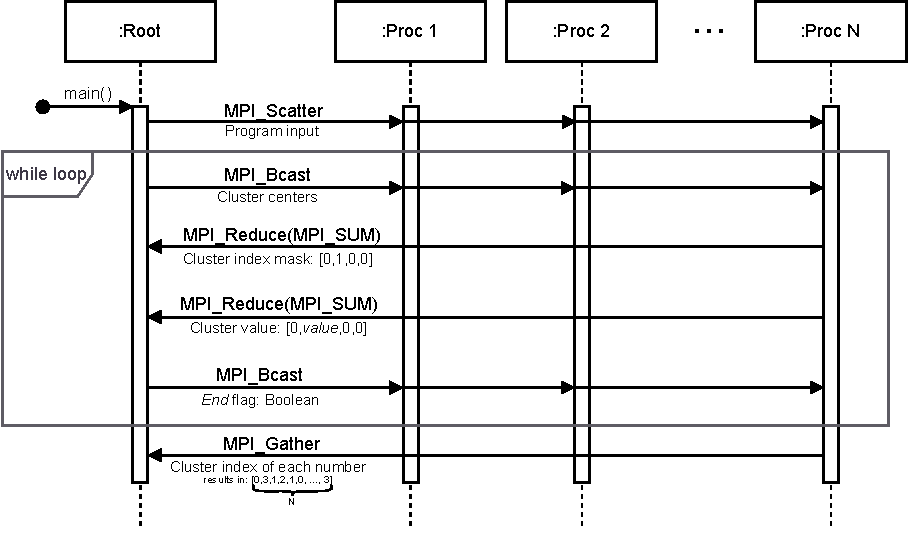
\includegraphics[width=1\textwidth]{seqdiag.pdf}
			\caption{The \texttt{MPI} communication protocol used for the program implementation.}
			\label{fig:seqdiag}
		\end{figure}

	\subsection{Analysis of the implementation}
	The implementation is restricted to single dimmension points, the number
	of clusters is set to $4$ and number of processes is equal to the
	input size $n$. The number of iteration is therefore $O(n)$ as presented
	in the article\;\cite{kmeans:iter}, where the author demonstrated this for
	k--means, where $k<5$ and points are one dimmensional. Each of the
	processes computes the minimal distance from each cluster and decides
	which is the minimum in constant time $O(1)$. This is due to the consatnt
	number of clusters. The sum--reduce is computed on N arrays of constant
	length 4 with time complexity $O(\log n)$. Based on this the final \textbf{time complexity} of the 4\,--\,means parallel implementation is: $O(n)\;\cdot\;(O(1) + O(\log n)) = O(n\cdot\log n)$.

	The space required for the implementation for each process is $O(n)$ for the sum--reduce operations, $O(1)$ for the minimal distance, $O(1)$ for 4\,--\,means centers and $O(1)$ for the boolean end flag. Therefore the \textbf{space complexity} is $O(n)$.

	The cost of the algorithm can be computed as follows: $c(n) = p(n)\;\cdot\;t(n)$, where the p(n) is number of processes for the input n (which is n in this case) and t(n) is the time complexity defined above. The \textbf{cost of the algorithm} is: $O(n^2\cdot\log n)$. The sequential algorithm implementationg would be $O(n^2)$, therefore the cost of parallel implementation is \textit{not} optimal.


\section{Conclusion}
The proposed parallel implementation of 4\,--\,means algorithm works as expected and even though it achieves speedup of $\frac{n}{\log n}$, its efficiency is $\frac{1}{\log n}$ which is not optimal.

\bibliographystyle{abbrv}
\bibliography{references}
\end{document}
